\documentclass{article}
\usepackage[utf8]{inputenc}
\usepackage{geometry}
\geometry{hmargin=2.5cm,vmargin=2.5cm}
\usepackage{mathtools} %\usepackage{align}
%\usepackage[french]{babel}
\usepackage{graphicx}
\usepackage{amsfonts}
\usepackage{bbold}
\usepackage{subcaption}

\title{SOD333 - Rapport}
\author{Paul-Antoine Leveilley \& Mila Rocco}
\date{Septembre 2022}

\begin{document}

\maketitle

\newpage
\tableofcontents
\newpage







\newpage
\section{TP1: Calcul d'une intégrale par méthode de Monte-Carlo, importance sampling.}
\subsection{Introduction}
Dans ce TP, on se propose de calculer une intégrale par méthode de Monte Carlo. De manière générale, la méthode de Monte Carlo
consisite à approcher l'intégrale : 
\[\mu = \int g(x)q(x)dx\] 
Ou $q$ est une densité, par l'estimateur : 
\begin{equation}
  \label{estim}
  \hat{\mu}_N = \frac{1}{N} \sum_{i=1}^N g(X_i)
\end{equation}
En effet, d'après la loi forte des grands nombres, 
\[\hat{\mu}_N\underset{p.s.}{\longrightarrow}\mu \] 

Pour illustrer cette méthode, nous allons estimer l'intégrale 
\[\int_0^1 cos(\frac{\pi x}{2})dx\]
Dont la valeur se calcule analytiquement, et vaut $\frac{2}{\pi}$ \\
Dans un premier temps, on mettra en oeuvre la méthode dite "naive" de Monte Carlo. Des considérations de minimisation de
la variance de l'estimateur nous conduirons à employer une méthode
plus précise. Ce sera l'objet de la deuxième partie.\\ 

 \subsection{Calcul par méthode de Monte Carlo naive}
Une première idée est de choisir la loi uniforme sur $[0,1]$, qui admet pour densité $q(x) = \mathbb{1}_{x \in [0,1]}$, ainsi que $g(x) = \cos (\frac{\pi x}{2})$
\subsubsection{Calcul préliminaire : variance de l'estimateur naif.}
Comme expliqué précédemment, la variance de l'estimation 
est un indicateur clé pour nous. On cherche à ce qu'elle soit la plus petite possible, 
de sorte à avoir une précision donnée sur le calcul de l'intégrale, en un nombre
minimum d'itérations. Employons nous donc à calculer cette variance pour (\ref{estim}). 
\begin{align*} 
   Var(\hat{\mu}_N) &= \frac1{N^2} \sum_{i=1}^N Var(g(X_i))\\ 
   &= \frac1{N^2}\times N Var(cos(\frac{\pi X}2)) \\ 
   &= \frac1{N} \left ( \int_0^1 cos^2(\frac{\pi x}2)dx - \left ( \int_0^1 cos(\frac{\pi x}2)dx \right )^2 \right )\\
   &= \frac1{N} \left ( \int_0^1 \frac{1+cos(\pi x)}{2}dx - 
    \frac4{\pi^2} \right )\\
   &= \frac1{N} \left ( \frac{1}{2} - 
    \frac4{\pi^2} \right )\\
 \end{align*}
\subsubsection{Simulations}
Dans l'intégralité de ce TP, on prendra $N=50$.
Pour réaliser cette estimation de $\mu$, nous simulons en machine
le tirage d'un échantillon $(X_{0},\textrm{...},X_{N})$ iid de loi uniforme sur $[0,1]$.
Ensuite, nous calculons une estimation de $\mu$ en utilisant l'estimateur (\ref{estim})
Nous réalisons ce calcul 10 fois, avec des échantillons différents. Le tableau (\ref{naif}) 
présente les résultat.
\begin{figure}[h!]
  \centering
  \caption{Calcul de l'estimation naive de $\mu$ pour 10 échantillons différents}
  \label{naif}
  \begin{tabular}{|*{11}{c|}}
    \hline 0.6685 & 0.67890& 0.69391& 0.59470& 0.69625&0.6424 & 0.64359& 0.61404& 0.65725& 0.63069 \\
    \hline
  \end{tabular}
\end{figure}

Nous observons que le résultat est assez proche de la valeur exacte de l'intégrale 
($\frac{2}{\pi} \approx 0.6366$). Cela dit, on constate également une forte variance des résultats de l'estimation. Nous avons cherché à 
estimer cette variance pour un nombre de $1000$ réalisations de l'estimation $\hat{\mu}_{N}$. Nous obtenons une variance empirique de $Var_{emp}(\hat{\mu}_{N})=0.00184$.
Ceci est conforme à ce qui est attendu. Le calcul de la partie précédente prédit en effet :  $Var(\hat{\mu}_{N}) \approx 1,89.10^{-3})$


\subsubsection{Théorème central limite : illustration}

Le théorème centrale limite prédit que l'erreur normalisée doit se comporter commme une loi 
normale centrée réduite pour $N \rightarrow \infty$. C'est à dire : 
\[\frac {\hat{\mu}_{N}-\mu }{\sigma /{\sqrt {N}}}\underset{\mathcal{L} }{\longrightarrow}\mathcal{N} (0,1)\]

Pour illustrer ceci, nous estimons la distribution de l'erreur renormalisée
par l'histogramme de 1000 réalisations de l'erreur renormalisée empirique. Nous présentons
ce résultat sur le graphique de la figure \ref{TP1_MC_TCL}, en superposant l'histogramme avec la représentation graphique de la densité de la gaussienne centrée réduite.
\begin{figure}[ht]
\centering
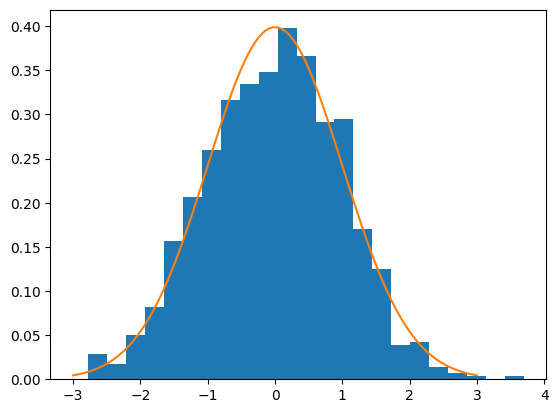
\includegraphics[width=0.4\textwidth]{TP1/MC_brute_TCL.png}
\caption{Distribution empirique de l'erreur renormalisée et densité de la gaussienne centrée réduite}
\label{TP1_MC_TCL}
\end{figure}

Nous constatons que, comme le prédit le TCL, l'erreur renormalisée possède une distribution proche d'une gaussienne centrée réduite.



\subsection{Echantillonage pondéré et réduction de la variance}
L'estimation de la partie précédente conduit à une grande variance du résultat.
Ce n'est pas satisfaisant et l'on peut faire mieux. En effet, quand nous estimons 
$\mu$ avec (\ref{estim}), nous donnons autant d'importance a chaque réalisation
de $X_{i}$ dans l'intégrale. Mais certains termes ont une contribution plus
importante dans le calcul. Ce sont les termes pour lesquels
$g(X_{i})$ est grand. Intuitivement, nous devons donc chercher à estimer "finement" les grandes valeurs de $gq$. Il faut donc 
tirer selon une densité la plus "proportionelle" possible à $gq$. C'est l'idée de l'échantillonage pondéré (préférentiel).\\

L'échantillonage pondéré consisite à remplacer $\hat{\mu}_{N}$ par : 
\[\tilde{\mu}_{N}= \frac1{N} \sum_{i=1}^N g(X_i)\frac{q(X_i)}{\Tilde{q}(X_i)}\]
Ou, $\tilde{q}$ est une densite et $(X_{i})_{1\leq i \leq n }$ est distribué selon une loi de densité $\tilde{q}$ 


En effet, dans ce cas, par loi forte des grands nombres, $\tilde{\mu}_{N}$ converge presque surement vers : 
\[\mathbb{E}^{\mathbb{Q}}[g(X)\frac{q(X)}{\tilde{q}(X)}]=\int_0^1 \frac{g(x)q(x)}{\Tilde{q}(x)} \Tilde{q}(x) dx = \int_0^1 g(x)q(x)dx = \mu \]
 Ou $\mathbb{E}^{\mathbb{Q}}$ désigne l'espérance sous la nouvelle probabilité $\mathbb{Q}$. Pour cette raison, on 
 appelle également cette technique "changement" de probabilité.

Maintenant, puisque c'est cela que nous cherchons à optimiser, calculons la variance de ce nouvel estimateur.

\begin{align*} 
   Var(\tilde{\mu}_N) &= \frac1{N^2} \sum_{i=1}^N Var \left( g(X_i)\frac{q(X_i)}{\Tilde{q}(X_i)} \right)\\ 
   &= \frac1{N} \left ( \int_0^1 \left (\frac{g(x)q(x)}{\Tilde{q}(x)} \right )^2 \Tilde{q}(x) dx  - \left ( \int_0^1 \frac{g(x)q(x)}{\Tilde{q}(x)} \Tilde{q}(x) dx \right )^2 \right )\\
   &= \frac1{N} \left ( \int_0^1 \frac{g^2(x)q^2(x)}{\Tilde{q}(x)} dx  - \left ( \int_0^1 g(x)q(x) dx \right )^2 \right )\\
   &= \frac1{N} \left ( \int_0^1 \frac{g^2(x)q^2(x)}{\Tilde{q}(x)} dx  - \mu^{2} \right )\\
   % &= \frac1{N} \left ( \int_0^1 \frac{cos^2(\frac{\pi x}2)}{\frac{\pi^2}{8} (1 -  x^2)} dx   - \mu^2 \right )\\
   % &\approx 1,98.10^{-5}\\
 \end{align*}
 On voit donc qu'en faisant le choix $\Tilde{q}=gq/ \int g(x)q(x)dx$, on obtient une variance nulle. C'est surprenant mais en fait c'est attendu,
 car l'intuition du changement de probabilité est d'échantillonner notre variable aléatoire selon
 une densité la plus "proportionelle" à $gq$. Le meilleur choix est donc sans surprise celui la. 
 Seulement, en pratique, on ne peut pas faire ce choix, car pour échantilloner selon $gq/\int gq$,
il faut être capable de calculer l'intégrale de $gq$ or c'est exactement ce que l'on 
cherche et que l'on suppose difficile à calculer. Dans la pratique, on choisit donc une
approximation de $gq/ \int gq$, un développement limité par exemple. Maintenant une autre question se
pose. Comment tirer une variable aléatoire ayant une loi à densité $\tilde{q}$? 

\subsubsection{Méthode du rejet}
 On voudrait simuler une variable aléatoire $X$
 selon une densité $f$.
 On suppose qu'il existe une densité $g$ telle que le rapport $\frac{f}{g}$ soit borné, disons, par $C$ et qu'on 
 sait simuler $Y$ selon $g$.

 La méthode du rejet consiste à :
 \begin{itemize}
   \item tirer $Y$ selon $g$ et $U$ uniforme sur $[0,1]$,
ce tant que $U>\frac{f(Y)}{Cg(Y)}$. 
   \item Des que ce n'est plus le cas (i.e. $U\leq \frac{f(Y)}{Cg(Y)}$ ), on pose $Z=Y$.
\end{itemize}
On peut prouver que $Z$ ainsi défini est une variable aléatoire à densité $f$.
On appelle probabilité d'acceptation le nombre :
\[P_{a}(C)=P(U\leq \frac{f(Y)}{Cg(Y)})\]
\subsubsection{Simulations de $\tilde{\mu}_{N}$}

Pour simuler $\mu$ grâce à $\tilde{\mu}_{N}$, on génère par méthode du rejet un échantillon de $N$
réalisation de $X$ selon la loi à densité $\tilde{q} = \frac{3}{2}(1 - x^2)  $. On a choisi cette
fonction a partir de $g(x)= \cos (\frac{\pi x}{2})$  en prenant un développement
limité en zero que l'on a translaté et renormalisé pour obtenir une densité à 
support dans $[0,1]$.

Cette fois ci, nous obtenons la valeur $\tilde{\mu}_{N}=0.63582$. Nous constatons une variance moindre. 

\begin{figure}
   \centering
   \caption{Représentation graphique de $g$ et de $\tilde{q}$}
   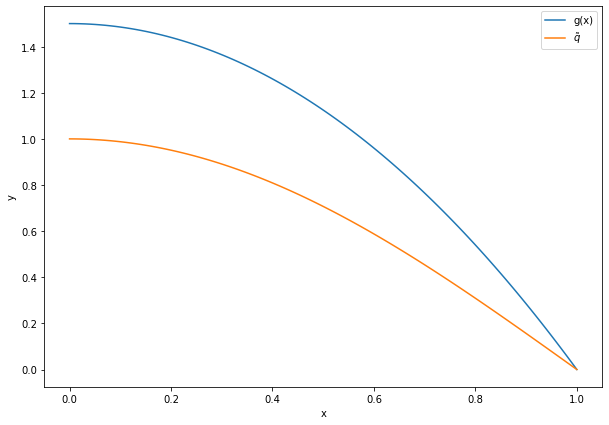
\includegraphics[width = 10cm]{TP1/gqtilde.png}
\end{figure}

Comme dans la partie précédente, nous estimons empiriquement la variance de $\tilde{\mu}_{N}$. Nous obtenons
$Var_{emp}(\tilde{\mu}_{N})=1.93.10^{-5}$, pour une valeur théorique de $Var_{\tilde{\mu}_{N}}\approx 1.98.10^{-5}$

Nous avons réalisé le même travail de comparaison de l'erreur renormalisée avec
la loi normale centrée réduite. Nous présentons cela en figure \ref{TCL_imp}. 

\begin{figure}[h!]
   \centering
   \label{TCL_imp}
   \caption{Comparaison de la densité de la loi $\mathcal{N}(0,1)$ et de l'erreur renormalisée de $\tilde{\mu}_{N}$ }
   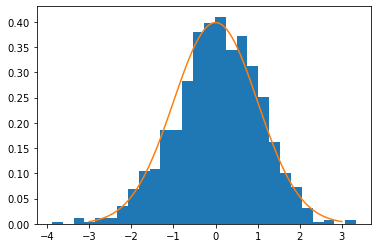
\includegraphics[width = 10 cm]{TP1/TCL_importance_sampling.png}
\end{figure}

Nous nous sommes intéressé à la probabilité d'acceptation dans notre méthode du rejet. En effet, la complexité de notre algorithme d'estimation dépend de cette probabilité.
On peut montrer qu'elle vaut
$P_{a}=\frac{1}{C}=\frac{1}{\tilde{q}(0)}= \frac{2}{3}$ dans notre cas. Par le calcul, nous obtenons une probabilité d'acceptation empirique de $0,667$, ce qui est attendu. Cela signifie qu'en moyenne, pour simuler 2 échantillons de $X$ selon
$\tilde{q}$, il nous faut de l'ordre de 3 opérations. 





\subsection{Conclusion}


Pour conclure, nous avons testé deux méthodes pour calculer notre intégrale par méthode de Monte Carlo. Une méthode dite naïve
qui donne lieu à une grande variance des résultat puis, une méthode plus rafinée qui fait
appel à un changement de probabilité. Grâce à cette méthode, nous avons pu réduire la variance d'un facteur presque 100 (83,7 pour être précis.) C'est donc très satisfaisant. Comparons le budget des deux méthodes. Pour rappel, nous avons
$N=50$. 
\begin{itemize}
   \item Méthode, naïve : pour obtenir une estimation, nous réalisons de l'ordre de N opération puisqu'il s'agit simplement de tirer $N$ réalisations d'une variable aléatoire et d'en faire la moyenne.
   \item Importance sampling : Cette fois ci, pour obtenir une estimation de $\mu$, nous avons besoin de N réalisations de $X$ selon $\tilde{q}$ mais pour tirer $X$ comme ceci, on fait en moyenne $\frac{3}{2}$ essais (inverse de la probabilité d'acceptation). In fine, on fait de l'ordre de $\frac{3}{2}N$ opérations, ce qui n'est pas beaucoup plus compte tenu du gain en variance. 
\end{itemize}

On conclut donc que l'échantillonage préférentiel est la méthode de 
choix lorsue l'on veut estimer une intégrale par méthode de Monte Carlo.
Ceci a des applications dans le calcul d'intégrales sur des espaces de grandes dimension. Cela sert en le filtrage bayésien, 
lorsque l'on propage des distributions conditionelles par exemple.

\clearpage

\section{TP2 : Filtre de Kalman: poursuite d'un mobile}
\subsection{Introduction}
Dans ce TP, nous allons simuler la trajectoire d'un mobile, et tenter de l'estimer à partir d'observations partielles et bruitées.

\subsubsection{Cadre général : filtre de Kalman}
On se donne un système linéaire du type :
\begin{equation*}
   \left\{
   \begin{array}{c}
      X_{k}=F_{k}X_{k-1}+f_{k}+W_{k} \\
      Y_{k}=H_{k}X_{k}+h_{k}+V_{k} \\
   \end{array}
   \right.
\end{equation*}
Ou les variables aléatoires suivent les hypothèses de la partie 3.1 de \cite{legland2008filtrage}, ce qui assure que 
le couple $(X_k,Y_k)$ forme un vecteur gaussien.
$X_k$ représente un système dont la dynamique est stochastique. $Y_k$ est une mesure de l'état du 
système. Le problème du filtrage consiste à estimer la loi de $X_k$ conditionnellement à l'information
disponible à l'instant $k$ : $Y_{0:k}$. Pour cela, comme les vecteurs sont gaussiens, il suffit de caractériser l'espérance et la covariance des lois conditionelles : 
\begin{equation*}
   \begin{array}{c}
      \hat{X}_{k}= \mathbb{E}[X_{k}| Y_{0:k}]\\
      P_k = \mathbb{E}\left[\left(X_k-\hat{X}_k\right)\left(X_k-\hat{X}_k\right)^{T}| Y_{0:k}\right]
   \end{array}
\end{equation*}
Il est pratique de définir également les quantités suivantes : 

\begin{equation*}
   \begin{array}{c}
      \hat{X}_{k}^{-}= \mathbb{E}[X_{k}| Y_{0:k-1}]\\
      P_k^{-} = \mathbb{E}\left[\left(X_k-\hat{X}_k\right)\left(X_k-\hat{X}_k\right)^{T}| Y_{0:k-1}\right]
   \end{array}
\end{equation*}

On montre alors que ces quantités obéissent aux relations de récurnce suivantes : 


\begin{align*}
   &\text{\underline{Etape de prédiction : }}\\
   &\hat{X}_{k}^{-}=F_k\hat{X}_{k-1} =f_{k}\\
   &P_{k}^{-}=F_{k}P_{k-1}F_{k}^{T}+Q_{k}^{W} \quad Q_{k}^{W}\text{ est la matrice de covariance de } (W_{k})\\
   &\text{\underline{Etape de correction : }}\\
   &\hat{X}_{k}= \hat{X}_{k}^{-}+K_{k}\left(Y_{k}-\left(H_{k}\hat{X}_{k}^{-}+h_k\right)\right)\\
   &P_k = (I-K_{k}H_{k})P_{k}^{-}
\end{align*}
Ou $K_k$ est le gain de Kalman. 
\[K_{k}= P_{k}^{-}H_{k}^{T}\left(H_{k}P_{k}^{-}H_{k}^{T}+Q_{k}^{V}\right)^{-1}\]
Avec $Q_{k}^{V}$ la matrice de covariance de $(V_k)$.


\subsection{Application, estimation d'une trajectoire}
Dans cette partie, on se donne le système suivant : un mobile de masse $m$ se déplace dans le plan. Il est décrit par son vecteur d'état, 
\[ X_t = \left (
   \begin{array}{c}
      x_t \\
      y_t \\
      \Dot{x_t} \\
      \Dot{y_t} \\
   \end{array} \right )\quad \forall t \in 0,...,T\]
Le mobile est soumis à une force aléatoire $(W_{t})_{t\in 0,...,T}$. Les équations de Newton nous donnent sa dynamique : 




\[ m \left (
   \begin{array}{c}
      \ddot{x_t} \\
      \ddot{y_t} \\
   \end{array} \right )
   =cW_t =c\left (
   \begin{array}{c}
      w_k^1 \\
      w_k^2 \\
   \end{array} \right )\ 
   \forall t \in [t_k, t_{k+1}]
\] Ou $c>0$ et $W_t$ est un bruit blanc gaussien centré réduit.

Après intégration en temps, la dynamique de $X_t$ s'écrit sous la forme matricielle suivante :
\[ X_t = \left ( 
   \begin{array}{cccc} %Fn
      1 & 0 & \delta t & 0 \\
      0 & 1 & 0 & \delta t \\
      0 & 0 & 1 & 0 \\
      0 & 0 & 0 & 1 \\
   \end{array} \right )
   \left ( 
   \begin{array}{cccc} %Xn-1
      x_{t-1} \\
      y_{t-1} \\
      \Dot{x}_{t-1} \\
      \Dot{y}_{t-1} \\
   \end{array} \right )
   + \left (
   \begin{array}{cc}
      \frac{c(\delta t)^2}{2m} & 0 \\
      0 & \frac{c(\delta t)^2}{2m} \\
      \frac{c\delta t}{m} & 0 \\
      0 & \frac{c\delta t}{m} \\
   \end{array} \right )
   \left (
   \begin{array}{c}
      w_t^1 \\
      w_t^2 \\
   \end{array} \right )
   = F X_{t-1} + G W_t
\]

Avec condition initiale: 
\[ m_0 = \mathbb{E}[X_0] = \left (
   \begin{array}{c}
      5000\ m \\
      5000\ m \\
      -20\ m/s \\
      20\ m/s \\
   \end{array} \right )
   ,\ P_0 = \left (
   \begin{array}{cccc}
      (2000\ m)^2 & 0 & 0 & 0 \\
      0 & (2000\ m)^2 & 0 & 0 \\
      0 & 0 & (5\ m/s)^2 & 0 \\
      0 & 0 & 0 & (5\ m/s)^2 \\
   \end{array} \right )
\]

Pour ce TP, nous prendrons les valeurs suivantes :
$$ \left\{
   \begin{array}{l}
      \delta t = 1\ seconde\\
      T = N \delta t = 200\ s \\
      c = 2\ m/s^2 \\
   \end{array} \right .$$



A chaque instant, on réalise une mesure partielle de l'état $X_t$, on ne mesure 
que la position. De plus, on suppose notre appareil de mesure bruité : 
\[ Y_t = \left ( 
   \begin{array}{cccc} %Fn
      1 & 0 & 0 & 0 \\
      0 & 1 & 0 & 0\\
   \end{array} \right )
   \left ( 
   \begin{array}{cccc} %Xn-1
      x_{t} \\
      y_{t} \\
      \Dot{x}_{t} \\
      \Dot{y}_{t} \\
   \end{array} \right )+
  \left (
   \begin{array}{c}
      v_t^{1} \\
      v_t^2 \\
      
   \end{array} \right )
\]

Ou $V_t = \left(v_t^{1},v_t^2\right)$ est un bruit blanc gaussien de matrice de covariance : 
\[Q_{k}^{V}= \left (
   \begin{array}{cccc}
      (50\ m)^2 & 0 \\
      0 & (50\ m)^2 \\
   \end{array} \right )
\]

\subsection{Simulations de la trajectoire et estimation par le filtre de Kalman}
Dans cette partie, nous simulons une trajectoire du mobile ainsi qu'une mesure bruitée de son état à chaque étape. Nous présentons cela 
en figure \ref{TP2_pos_vit}. 
\begin{figure}[!htb]
\centering
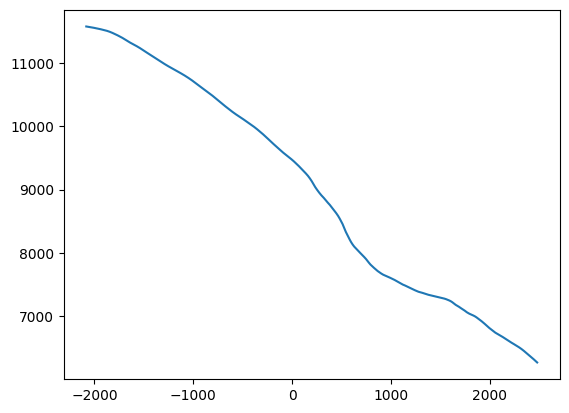
\includegraphics[width=0.4\textwidth]{TP2/position_réelle.png}
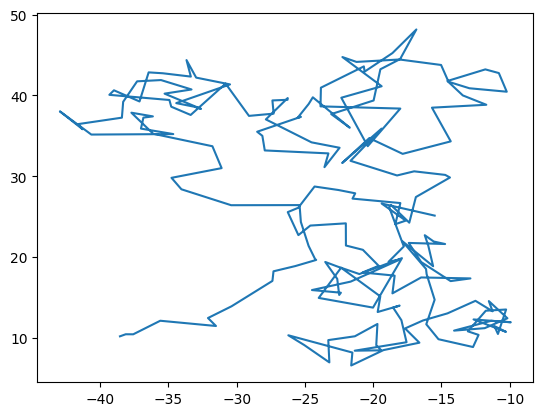
\includegraphics[width=0.4\textwidth]{TP2/vitesse_reelle.png}
\caption{Simulation d'une trajectoire du mobile. Position à gauche et vitesse à droite.}
\label{TP2_pos_vit}
\end{figure}

Ce qui est intressant avec le filtre de Kalman est que l'on connait la covariance de la distribution
conditionelle a chaque étape. On peut donc tracer des 
intervalles de confiance à 95\%. C'est ce que nous présentons en figure \ref{ellipse}.

\begin{figure}[!htb]
   \centering
   \caption{Trajectoire estimée par le filtre de Kalman et intervalles de confiance à 95\% associés.}
   \label{ellipse}
   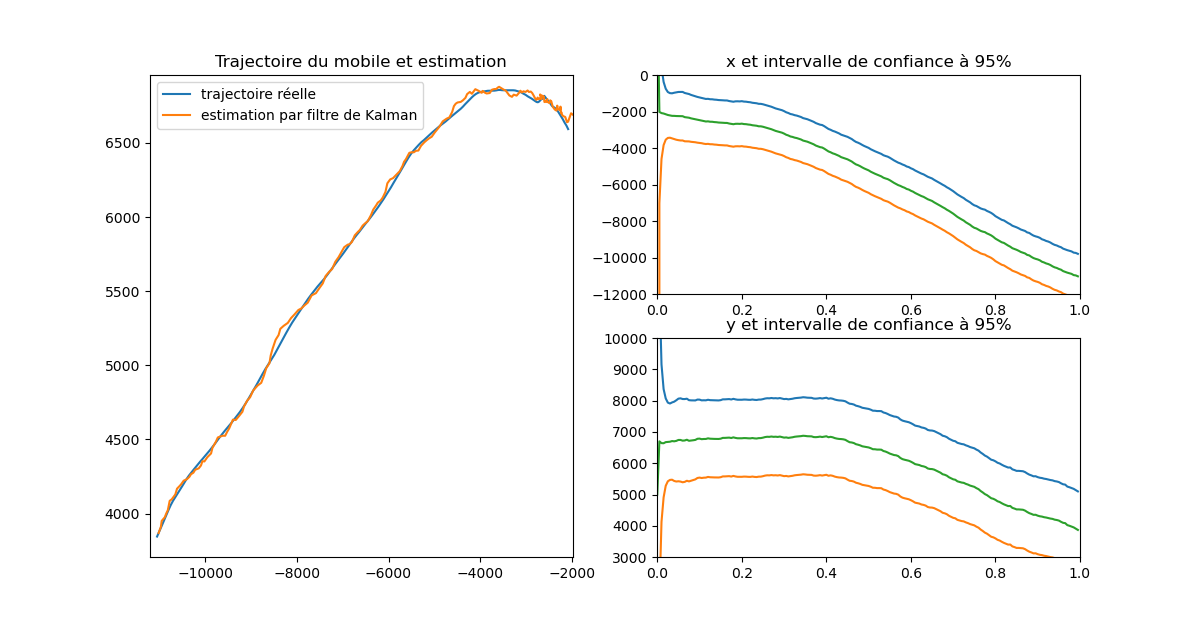
\includegraphics[width = 18cm]{TP2/filtre_kalman.png}
\end{figure}

D'ailleurs, puisque la méthode du filtre de Kalman fournit des matrices de covariance, on 
peut tracer des ellipses de confiance à 95\% autour de l'estimation de la trajectoire
de $X$ c'est ce que nous présentons en figure \ref{ellipse_conf}. 

\begin{figure}[!htb]
   \centering
   \caption{Trajectoire estimée par le filtre de Kalman et ellipses de confiance à 95\% associées.}
   \label{ellipse_conf}
   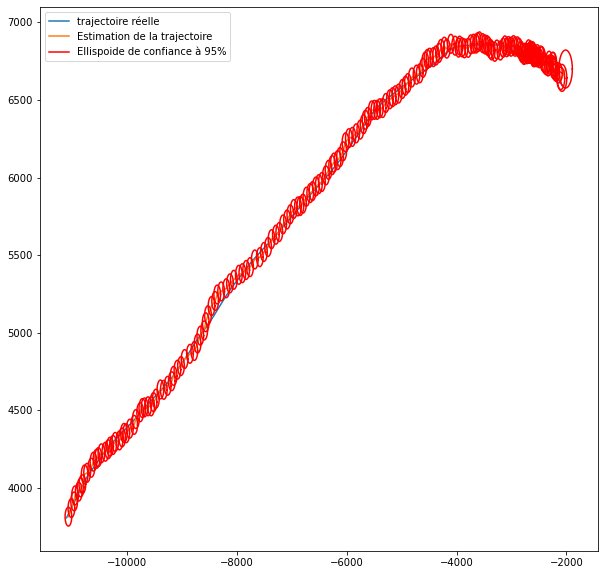
\includegraphics[width = 10cm]{TP2/ellipses_conf.png}
\end{figure}

On constate qu'au départ, il existe une grande incertitude sur la position du mobile.
Cette incertitude décroit pendant les premières itérations, jusqu'à ce qu'elle se stabilise autour d'une certaine valeur.
Il est intéressant de noter que les ellipses de confiance à 95\% autour de 
l'estimation de la trajectoire contiennent bien les points de la trajectoire réelle,
comme attendu.
\subsection{Conclusion}



\clearpage


\section{TP3 : Borne de Cramer Rao.}
\subsection{Introduction}
\subsubsection{Borne de Cramer Rao pour un problème de filtrage}

Dans ce TP, on se propose de calculer une borne de Cramer Rao pour un problème de filtrage. Le cadre général est le suivant.
On se donne un système  $(X_{k})_{k\geq 0}$ sujet à une certaine dynamique,
ainsi qu'une série de mesures bruitées $(y_{k})_{k \geq 0}$ (bruit gaussien de variance $\sigma_{k}^{2}$) : 
\[\left\{\begin{array}{ll}
   X_{k+1} = \phi(k,k+1)X_{k} \\
   y_{k}=h_{k}(X_{k})+\epsilon_{k}
\end{array}\right. \]

Avec $X_{0} \sim  \mathcal{N} (X_{\nu},P_{0})$. On peut montrer que la matrice d'information ralative à l'instant $k$ vérifie
la relation de récurence suivante : 

\[ J_{k} = \frac{1}{\sigma_{k}}\left(\frac{\partial h_{k}}{\partial X_{k}}\right)\left(\frac{\partial h_{k}}{\partial X_{k}}\right)^{T}+\left(\frac{\partial X_{k-1}}{\partial X_{k}}\right)^{T}J_{k-1}\left(\frac{\partial X_{k-1}}{\partial X_{k}}\right)\]

Avec $J_{0}=P_{0}^{-1}$ et $\phi(k,k+1)=\frac{\partial X_{k+1}}{\partial X_{k}}$.
La borne de Cramer Rao à l'instant $k$ est alors égale à l'inverse de la matrice d'information : 
\[BCR_{k}= J_{k}^{-1}\]

\subsubsection{Application : poursuite de bateau}
Nous étudions le système suivant : un bateau émetteur de bruit se déplace dans le plan de manière rectiligne uniforme. 
Un bateau observateur mesure la direction d'ou lui parvient le bruit, plus précisément, il mesure l'angle $\theta_{k}$ que fait cette direction avec l'horizontale, ce toute les secondes pendant 100s. Le bateau observateur se déplace également en ligne droite à vitesse constante.
L'état de l'émeteur est donné par sa position et sa vitesse : $X_{k} = (x_{k},y_{k},\dot{x}_{k},\dot{y}_{k})$, sa matrice de transition est :
\[\phi(k,k+1) = \phi =  \begin{pmatrix}
  1 & 0 & T & 0 \\
  0 & 1 & 0 & T \\
  0 & 0 & 1 & 0 \\
  0 & 0 & 0 & 1 
  \end{pmatrix}\]

Pour pouvoir discriminer entre différentes
trajectoires possibles, le bateau doit virer de bord à un certain moment. Si ça n'est pas le cas, on peut vérifier que des trajectoires différentes peuvent donner lieu à des mesures d'angle identiques.
Pour simplifier l'étude, on suppose que le bateau vire de bord toujours au même moment : au milieu du trajet. Le bateau observateur choisit l'angle $\varphi $ duquel il tourne. Chaque choix de $\varphi$ 
conduit à une précision différente de l'estimation de la trajectoire  de l'émeteur.
La question est donc la suivante : quel choix de $\varphi$ est le meilleur pour estimer la trajectoire de l'émeteur?
\\
Pour répondre à cette question, nous allons simuler la dynamique de l'éméteur et de l'observateur. Grâce à ces dynamiques, nous allons
calculer le gradient de la fonction d'observation et nous allons en déduire la matrice d'information.
Dans notre cas, la fonction d'observation est l'angle que fait la direction d'observation avec l'horizontale. 
En terme de l'abscisse et de l'ordonnée de l'éméteur et de l'observateur, cette fonction s'écrit : 
\[h_{k}(X_{k})=\arctan \left(\frac{y_{k}-y_{k}^{o}}{x_{k}-x_{k}^{o}}\right)\]

En inversant la matrice d'observation, on obtiendra la borne de Cramer Rao, sous forme d'une matrice carrée d'ordre 4.
On cherchera ensuite la valeur de $\varphi$ qui minimise le critère : $\sqrt{\sigma_{x_{n}}^{2}+\sigma_{y_{n}}^{2}}$

\subsubsection{Calcul du gradient de $h_{k}$ par rapport à $X_{k}$}
Déjà, on voit facilement que : 
\[\frac{\partial h_{k}}{\partial \dot{x}_{k}} = 0 \] et :
\[\frac{\partial h_{k}}{\partial \dot{y}_{k}} = 0 \]
Ensuite, par le calcul, on a que : 
\[\frac{\partial h_{k}}{\partial x_{k}}=\frac{y_{k}^{o}-y_{k}}{\left(x_{k}-x_{k}^{o}\right)^{2}\left(1+\left(\frac{y_{k}-y_{k}^{o}}{x_{k}-x_{k}^{o}}\right)^{2}\right)}\]
et :

\[\frac{\partial h_{k}}{\partial y_{k}}= \frac{1}{\left(x_{k}-x_{k}^{o}\right)\left(1+\left( \frac{y_{k}-y_{k}^{o}}{x_{k}-x_{k}^{o}}  \right)^{2}\right)}\]
\subsection{Simulations des dynamiques de l'observateur et de l'émetteur}
Nous avons simulé la dynamique du système pour différents changements de cap de l'observateur, avec les paramètres du tableau \ref{paramètres}.
 Nous obtenons les tracés de la figure \ref{trajectoire}


\begin{figure}[h!]
  \centering
  \caption{Paramètres pour la simulation}
  \label{paramètres}
  \begin{tabular}{|*{11}{c|}}
    \hline Horizon temporel & $T = 1$ \\
    \hline Nombre de mesures  & $N=100$ \\
    \hline Ecart type du bruit & $\sigma_{k}=1^{\circ}$\\
    \hline Vitesse de l'observateur & $V_{o}=10 m.s^{-2}$\\
    \hline Position initiale de l'observateur &  $(x_{0}^{o},y_{0}^{o})=(0,0)$ m\\
    \hline Vitesse de l'émetteur & $V_{e} = 5 m.s^{-2}$\\
    \hline Cap de l'émetteur & $\alpha =-20^{\circ}$\\
    \hline Position initiale de l'émetteur & $(x_{0},y_{0})=(2000,2000)$\\
    \hline Incertitude initiale sur la position de l'émetteur & $P_{0}=diag(1000,1000,10,10)^{2}$\\
    \hline
  \end{tabular}
\end{figure}


 \begin{figure}[h!]
  \centering
  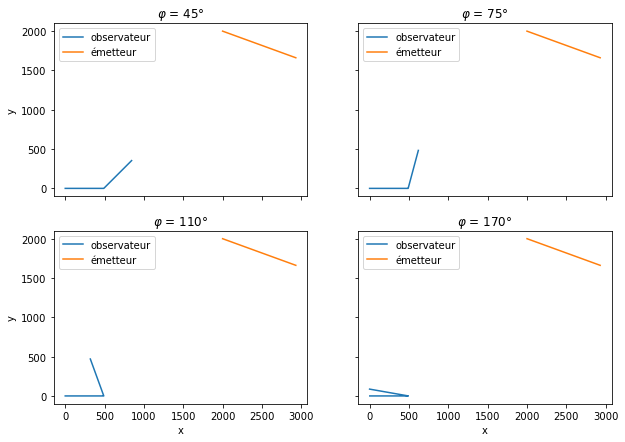
\includegraphics[width = 15cm]{TP3/trajectoires.png}
  \label{trajectoire}
  \caption{Trajectoires de l'émetteur et de l'observateur pour différentes valeurs de l'angle $\varphi$}
\end{figure}

Grâce à ces dynamiques, nous sommes capables de calculer la Borne de Cramer Rao associée à cet estimateur de la position de l'émetteur. 
Nous présentons ces résultat en figure \ref{cramerrao}. 

\begin{figure}[h!]
  \centering
  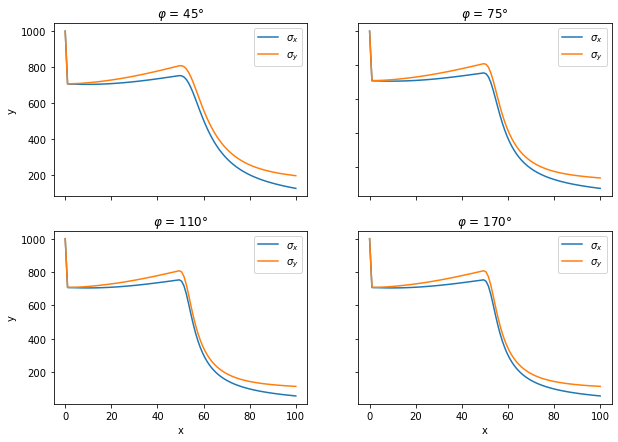
\includegraphics[width = 15cm]{TP3/cramer rao.png}
  \caption{Borne de Cramer Rao pour l'abscisse et l'ordonnée de la position de l'émetteur au cours du temps, pour différentes valeurs de $\varphi$}
  \label{cramerrao}
\end{figure}

\subsection{Optimisation de la valeur de $\varphi$}
Pour trouver la valeur de $\varphi$ optimale, nous avons simplement testé toutes les valeurs entre $0^{\circ}$ et $360^{\circ}$, avec un pas de 
$1^{\circ}$. Nous avons trouvé une valeur optimale de $\varphi = 109^{\circ}$, ce qui correspond à la trajectoire représentée en figure
\ref{opti_}. La borne de Cramer Rao associée est représentée en figure \ref{crameropti}. Le critère associé est un écart type sur la position de 128m.

\begin{figure}[h!]
   \centering
   \begin{minipage}[t]{8cm}
       \centering
       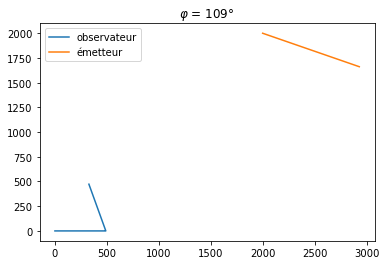
\includegraphics[width=7cm]{TP3/trajopti.png}
       \caption{Trajectoire optimale pour l'observateur}
       \label{opti_}
   \end{minipage}
   \begin{minipage}[t]{8cm}
       \centering
       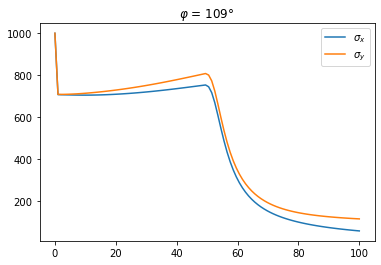
\includegraphics[width=7cm]{TP3/crameropti.png}
       \caption{Borne de Cramer Rao pour la trajectoire optimale}
       \label{crameropti}
   \end{minipage}
\end{figure}

\subsection{Conclusion}
En conclusion, ce TP nous aura permis de voir comment la Borne de Cramer Rao permet de réaliser le choix d'une stratégie pour 
optimiser la précision sur l'estimation de état d'un système, grâce à la seule connaissance d'un modèle à priori.

\clearpage


\section{TP4: Navigation par corrélation de terrain - filtre particulaire}
\subsection{Introduction}
Ce TP est l'aboutissement du tout ce qui précède. Dans ce TP, nous allons 
implémenter le filtre particulaire pour un problème de filtrage non linéaire : la navigation par corrélation de terrain. 
La première partie présente ce qu'est le filtre particulaire. La deuxième partie discute de 
notre problème spécifique et de l'implémentation du filtre particulaire dans ce cas. 
\subsection{Filtre optimal et filtre particulaire}
\subsubsection{Filtre optimal}
Rappelons les équations du filtrage :

On considère une chaîne de Markov $(X_{n})_{n \geq 0}$ à valeurs dans $\mathbb{R}^d$, de loi initiale $\pi_0$, i.e. $\pi_0(dx_{1:d})=P(X_0 \in dx_{1:d})$, et de noyau de transition 
$Q_{n}(x_{n-1},dx_{1:d})= P(X_n \in dx_{1:d} \vert X_{n-1}=x_{n-1} )$. 
On considère les observations bruitées $Y_n = h(X_n)+ V_n \in \mathbb{R}^q$. On suppose que les 
$V_n$ sont iid et a densité $g$ par rapport à la mesure de Lebesgue. On suppose de plus que $V_n \perp X_0$. On introduit la fonction de vraissemblance  
$\psi_n(x)=g((Y_n-h(x)))$ c'est donc une fonction aléatoire qui n'est connue que lorsque l'on a la n ème réalisation de $Y$. La fonction de vraissemblance mesure la cohérence entre le point de l'espace d'état $x$
et l'observation courante. \\
On appelle filtre optimal la suite de mesures de probabilité suivante : $(\Pi_n)_{n \geq 0}$ ou $\Pi_0 = \pi_0$ et $\Pi_n(dx_{1:d})= P(X_n \in dx_{1:d} \vert Y_{0:n})$. Il est également utile d'introduire la suite 
$\Pi_{n \vert n-1} = P(X_n \in dx_{1:d} \vert Y_{0:n-1})$. 
On montre que : 

\begin{align*}
   \Pi_n(dx_{1:d}) &=P(X_n \in dx_{1:d} \vert Y_{0:n})\\
                  &=\frac{P(X_n \in dx_{1:d}, Y_n \in dy_{1:q} \vert Y_{0:n-1})}
                  {P(Y_n \in dy_{1:q} \vert Y_{0:n-1})}\\
                  &= \frac{P(Y_n \in dy_{1:q} \vert X_n = x_n)P(X_n \in dx_{1:d} \vert Y_{0:n-1})}
                  {P(Y_n \in dy_{1:q} \vert Y_{0:n-1})}\\
                  &= \frac{P(Y_n \in dy_{1:q} \vert X_n = x_n)P(X_n \in dx_{1:d} \vert Y_{0:n-1})}
                  {\displaystyle{\int_{x_n \in \mathbb{R}^d} P(Y_n \in dy_{1:q} \vert X_n = x_n)P(X_n \in dx_{1:d} \vert Y_{0:n-1}) \, }}\\
\end{align*}
On peut voir que : 
\begin{align*}
   P(Y_n \in dy_{1:q} \vert X_n =x_n)&=P(V_n \in dy_{1:q}-h(x_n) \vert X_n = x_n)\\
   &=g(Y_n-h(x_n))dy_{1:q}\\
\end{align*}
de sorte que : 
\[\Pi_n(dx_{1:d}) = \frac{\psi_n(x_n)\Pi_{n \vert n-1}(dx_{1:d})}{\displaystyle{\int_{x_n \in \mathbb{R}^d} \psi_n(x_n)\,\Pi_{n \vert n-1}(dx_{1:d})}}\]
Cette opération s'appelle le produit projectif de $\Pi_{n \vert n-1}$ par $\psi$, et se note : $\Pi_{n} = \psi_n \boldsymbol{\cdot} \Pi_{n \vert n-1}$
\newline
Il reste donc à voir comment passer de $\Pi_{n-1}$ à $\Pi_{n \vert n-1}$.
\begin{align*}
   \Pi_{n \vert n-1}((dx_{1:d})_n) &= P(X_n \in (dx_{1:d})_{n}\vert Y_{0:n-1})\\
   &=\displaystyle{\int_{x_{n-1}\in \mathbb{R}^d} \,P(X_n \in (dx_{1:d})_n,X_{n-1} \in (dx_{1:d})_{n-1} \vert Y_{0:n-1})}\\
   & = \displaystyle{\int_{x_{n-1}\in \mathbb{R}^d} \,
    P(X_n \in (dx_{1:d})_n \vert X_{n-1}, Y_{0:n-1}) 
    \Pi_{n}((dx_{1:d})_{n-1})}\\
\end{align*}
Mais $X_n$ est une chaîne de Markov donc, en particulier, sa loi ne dépend pas des observations passées $Y_{0:n-1}$. on a alors : 
\begin{align*}
   \Pi_{n \vert n-1}((dx_{1:d})_n) & =  \displaystyle{\int_{x_{n-1}\in \mathbb{R}^d} \,
   P(X_n \in (dx_{1:d})_n \vert X_{n-1}) 
   \Pi_{n}((dx_{1:d})_{n-1})}\\
   &=\displaystyle{\int_{x_{n-1}\in \mathbb{R}^d}\Pi_{n-1}((x_{1:d})_{n-1})\,Q_n(x_{n-1},(dx_{1:d})_n)}\\
   &=(\Pi_{n-1}Q_n)((dx_{1:d})_n)
\end{align*}
On appelle cette opération le "transport" de la mesure $\Pi_{n-1}$ par le noyau $Q_n$.
\\
On peut résumer le filtre optimal par le schéma suivant : 

\[\Pi_{n-1} \xrightarrow[prediction]{} \Pi_{n \vert n-1} = (\Pi_{n-1}Q_{n})\xrightarrow[correction]{}  \Pi_{n}=\psi_n \boldsymbol{\cdot}\Pi_{n \vert n-1}\]
\subsubsection{Filtre particulaire}

En pratique, le filtre optimal est très compliqué à calculer car les étapes de prédiction et de correction font intervenir des intégrales dans des espaces à (possiblement) grande dimension. On préfère alors utiliser le filtre particulaire.
L'idée du filtre particulaire est d'approcher le filtre optimal par des méthodes de Monte Carlo.
Le filtre particulaire repose sur l'idée de mesure empirique. On appelle mesure empirique associée à un échantillon $(X_0, ... , X_n)$ iid suivant la loi 
$\Pi$ la mesure $S^N(\Pi)= \frac{1}{N}\sum_{i=1}^{N} \delta_{X_i}$ ou $\delta_x$ désigne la mesure de Dirac en $x$. 
Il faut bien voir qu'étant donné une mesure $\Pi$, $S^{N}(\Pi)$ est une mesure aléatoire. Elle dépend de l'échantillon $(X_0, ... , X_n)$.
Le filtre particulaire consiste alors en les opérations suivantes : 
\[\Pi_{n-1}^N \xrightarrow[prediction ~ echantillonee]{} \Pi_{n \vert n-1}^N = S^N(\Pi_{n-1}^NQ_{n})\xrightarrow[correction]{}  \Pi_{n}^N=\psi_n \boldsymbol{\cdot}\Pi_{n \vert n-1}^N\]
Regardons en détail les étapes de prédiction et de correction pour comprendre l'intérêt du filtre particulaire.
\paragraph{correction}
A cette étape, on dispose de $\Pi^{N}_{n \vert n-1} = \frac{1}{N}\sum_{i=1}^{N} \delta_{X_{n \vert n-1}^{i,N}}$,
ou $(X_{n \vert n-1}^{1,N},...,X_{n \vert n-1}^{N,N} )$ est un échantillon iid distribué selon 
$\Pi_{n}^{N}Q_{n}$. 
On peut alors calculer $\Pi_{n}^{N}$ : 
\begin{align*}
   \Pi_{n}^{N}(dx_{1:d}) &= \psi_n \boldsymbol{\cdot} \Pi_{n \vert n-1}^N\\
   &=\frac{\psi_n(x)\Pi_{n \vert n-1}^N(dx_{1:d})}{\displaystyle{\int_{x \in \mathbb{R}^d} \psi_n(x)\,\Pi_{n \vert n-1}^N(dx_{1:d})}}\\
   &=\frac{\displaystyle{\sum_{i=1}^{N}\psi_n(X_{n \vert n-1}^{i,N})\delta_{X_{n \vert n-1}^{i,N}}}}{\frac{1}{N}\displaystyle{\sum_{j=1}^{N} \psi_{n}(X_{n \vert n-1}^{j,N})}}\\
\end{align*}
On pose alors : 
\[\omega_{n}^i= \frac{\psi_n(X_{n \vert n-1}^{i,N})}{\frac{1}{N}\displaystyle{\sum_{j=1}^{N} \psi_{n}(X_{n \vert n-1}^{j,N})}}\]
De sorte que :
\[\Pi_{n}^{N}= \sum_{i=1}^{N}\omega_{n}^{i}\delta_{X_{n \vert n-1}^{i,N}}\]
On voit donc que l'étape de correction devient une étape de pondération de chaque particule par un poids proportionnel à sa vraissemblance.
\paragraph{prédiction échantillonée}
A l'étape $n$, on a $\Pi_{n}^N= \sum_{i=1}^{N}\omega_n^i\delta_{X_{n \vert n-1}^{i,N}}$
On peut alors calculer le transport de la mesure $\Pi_n^N$ par le noyau $Q_{n+1}$ : 
\begin{align*}
   (\Pi_n^N Q_{n+1})(dx_{1:d}) &=\displaystyle{\int_{y_{1:d}\in \mathbb{R}^d}\,\Pi_n^N(dy_{0:d})Q_{n+1}(y_{1:d},dx_{1:d})}\\
   &=\displaystyle{\int_{y_{1:d}\in \mathbb{R}^d}\,\sum_{i=1}^N \omega_n^i \delta_{X_{n \vert n-1}^{i,N}}Q_{n+1}(y_{1:d},dx_{1:d})}\\
   &=\sum_{i=1}^N \omega_n^i Q_{n+1}(X_{n \vert n-1}^{i,N},dx_{1:d})
\end{align*}
Ecris sous cette forme, on constate que $(\Pi_n^N Q_{n+1})$ est un mélange de probabilités. Or il est facile de générer
un échantillon selon un mélange de probabilités. On peut faire comme ceci : 
\begin{itemize}
   \item Générer $I$ selon $P(I=i)=\omega^i_n$
   \item Générer $X$ selon $Q_{n+1}(X_{n\vert n-1}^{I,N},\cdot)$
\end{itemize}
Cela revient à séléctionner les particules selon leur poids (plus le poids d'une 
particule est grand, plus on a de chance de la tirer), puis à faire evoluer la particule 
selon la dynamique de la chaîne de Markov.
\subsubsection{Dynamique déterministe}
Le cas d'une dynamique déterministe $X_{n+1}=f(X_n)$ est un peu embêtant. En effet, l'étape de prédiction
échantillonnée fait une séléction des particules. Si aucun bruit n'est ajouté par l'évolution, la séléction va finir par "tuer" la diversité des particules. 
Dans ce cas (et c'est le cas qui se présente pour nous dans le TP), il est nécéssaire de régulariser la mesure $\Pi_n^N$ (à l'étape de prédiction).
Concrètement, on remplace $\Pi_n^N$ par :
\[\tilde{\Pi}_n^N=\sum_{i=1}^N \omega_n^i K\left(\frac{\boldsymbol{\cdot}-X_{n \vert n-1}^{i,N}}{h}\right) \]  
Ou $K$ est un noyau (Gaussien, Epanechikov,...) et $h$ est un paramètre qui contrôle la "finesse" de la régularisation. Il existe un choix de $h$ qui minimise l'erreur quadratique moyenne entre la mesure discrète et la mesure régularisée, notons le $h_{opt}$.
\newline
L'étape de prédiction échantillonnée devient alors : 
\begin{itemize}
   \item Générer $I$ selon $P(I=i)=\omega^i_n$
   \item Générer $\epsilon$ selon $K$.
   \item Poser $\tilde{X}^{i,N}_{n \vert n-1}=X^{I,N}_{n \vert n-1} + h_{opt}\Gamma_k \epsilon$. Avec, $\Gamma_k^{T}\Gamma_k=Cov\left((X_{n \vert n-1}^{i,N})_{i\in \left\{1,...,N\right\}}\right) $
   \item Faire évoluer la particule : $ X_{n}^{i,N}= f(\tilde{X}^{i,N}_{n \vert n-1})$
\end{itemize}

\subsection{Navigation par corrélation de Terrain}
Le problème de la navigation par corrélation de terrain est le suivant : 
un avion se déplace en ligne droite à vitesse constante (horizontale). Disons qu'à un moment,
il perd son signal GPS et se retrouve "perdu", c'est à dire qu'il y a une incertitude sur son état (position/vitesse). Dans ce cas, il 
existe un moyen pour l'avion de retrouver sa position avec une précision acceptable. En effet, les avions embarquent dans leur ordinateurs de bord
des modèles numériques de terrain, c'est a dire une carte de l'altitude du sol en fonction de la position. En effectuant des mesures d'altitude et en "corrélant" ces 
mesures au modèle de terrain, l'avion peut se retrouver. Naturellement, ces mesures sont bruitées. On retrouve en fait un problème de filtrage avec les paramètres suivants :
\begin{equation*}
   X_k = (x_k,y_k,z_k,\Dot{x}_k,\Dot{y}_k,\Dot{z}_k)^T\\
\end{equation*}
\begin{equation*}
   \left\{\begin{array}{c}
      X_k = \Phi X_{k-1} \\
      Y_k=h(X_k)+\epsilon_k = Z_k -h_{MNT}(x_k,y_k)+\epsilon_k \\
   \end{array}\right.
\end{equation*}
\begin{figure}[h!]
   \centering
   \label{MNT}
   \caption{Navigation par corrélation de terrain, illustration}
   \includegraphics[width = 8 cm]{TP4/MNT.png}
\end{figure}
Avec,
\[\Phi = \begin{pmatrix}
            1&0&0&dt&0&0\\
            0&1&0&0&dt&0\\
            0&0&1&0&0&dt\\
            0&0&0&1&0&0\\
            0&0&0&0&1&0\\
            0&0&0&0&0&1\\
         \end{pmatrix}
\]
Dans le TP, $h_{MNT}$ est un tableau de nombres donné.

Comme discuté précédemment, la dynamique de ce problème est déterministe (l'avion se déplace en ligne droite, a vitesse constante). 
Il faut dont mettre en oeuvre la technique de régularisation. Nous avons choisi d'utiliser un noyau Gaussien.
Simplement, cette étape est assez coûteuse. Pour s'épargner du temps de calcul, on 
ne la pratique que lorsque l'on détecte que la diversité de l'échantillon de particules est 
trop faible. Quand la condition $N_eff = \frac{1}{\sum_{i=1}^{N}\omega_i^2} \leq N_{th}=Coeff \times N$, on procède au rééchantillonage.
En pratique, un bon choix est $Coeff = 0.4$.

Les paramètres du problème sont résumés dans le tableau \ref{paramètres2} : 


\begin{figure}[h!]
   \centering
   \caption{Paramètres pour la simulation}
   \label{paramètres2}
   \begin{tabular}{|*{11}{c|}}
     \hline Horizon temporel & $T = 720 s$ \\
     \hline Vitesse avion & $v=300 km.h^{-1}$\\
     \hline Cap de l'avion & $\theta = 45^\circ$\\
     \hline Etat initial & $X_0 =\left(150,150,8,v \cos(\theta),v \sin(\theta),0\right) km $\\ 
      \hline dt  & $dt = 1 s$ \\
      \hline Ecart type bruit mesure & $\sigma_{mes}=30 m$\\
      \hline Incertitude initiale position(forme $P_0$)& $(\sigma_x,\sigma_y,\sigma_z)=(3000,3000,500) m$\\
      \hline Incertitude initiale vitesse (forme $P_0$)&$(\sigma_{v_{x}},\sigma_{v_{y}},\sigma_{v_{z}})=(5,5,5) m.s^{-1}$\\
      \hline Nombre de particules & $N=5000$ \\
      \hline
   \end{tabular}
 \end{figure}
 
 Pour initialiser l'algorithme, on tire une position initiale "fausse", uniformément autour de $X_0$, dans les intervalles
 $X_0 \pm \sigma_{x,y,z}$, puis on tire les particules initiales autour de cette fausse position, selon une distribution gaussienne de matrice de covariance $P_0$.

 La figure \ref{traj} présente la trajectoire de l'avion. La figure \ref{mesure_alt} montre les mesures
 que fait l'avion le long d'une trajectoire (avec et sans le bruit). La figure \ref{particu} montre 
 le tirage initial des particules.

 \begin{figure}[h!]
   \centering
   \caption{Trajectoire de l'avion}
   \label{traj}
   \includegraphics[width= 10 cm]{TP4/Traj.png}
 \end{figure}

 \begin{figure}[h!]
   \centering
   \caption{Trajectoire de l'avion}
   \label{mesure_alt}
   \includegraphics[width= 14 cm]{TP4/mesure.png}
 \end{figure}

 \begin{figure}[h!]
   \centering
   \caption{Tirage initial des particules}
   \label{particu}
   \includegraphics[width= 10 cm]{TP4/tirage_init.png}
 \end{figure}

 \paragraph{Résultats}
 Apres quelques efforts, nous avons été capables de faire fonctionner le 
 filtre particulaire. La figure \ref{navigation} présente l'évolution des
 particules. On constate bien que le groupe de particules se concentre autour de la 
 vraie position de l'avion. De plus, on observe clairement les étapes de redistribution,
 et l'on comprend bien comment elles agissent pour explorer l'espace des états à partir
 des positions pertinentes connues.
 

 \begin{figure}[h!]
   \centering
   \begin{minipage}[t]{4cm}
       \centering
       \includegraphics[width=4cm]{TP4/10.png}
   \end{minipage}
   \begin{minipage}[t]{4cm}
       \centering
       \includegraphics[width=4cm]{TP4/20.png}
   \end{minipage}
   \begin{minipage}[t]{4cm}
      \centering
      \includegraphics[width=4cm]{TP4/30.png}
  \end{minipage}
  \begin{minipage}[t]{4cm}
   \centering
   \includegraphics[width=4cm]{TP4/40.png}
\end{minipage}
\begin{minipage}[t]{4cm}
   \centering
   \includegraphics[width=4cm]{TP4/50.png}
\end{minipage}
\begin{minipage}[t]{4cm}
   \centering
   \includegraphics[width=4cm]{TP4/60.png}
\end{minipage}
\begin{minipage}[t]{4cm}
   \centering
   \includegraphics[width=4cm]{TP4/70.png}
\end{minipage}
\begin{minipage}[t]{4cm}
   \centering
   \includegraphics[width=4cm]{TP4/80.png}
\end{minipage}
\begin{minipage}[t]{4cm}
   \centering
   \includegraphics[width=4cm]{TP4/90.png}
\end{minipage}
\begin{minipage}[t]{4cm}
   \centering
   \includegraphics[width=4cm]{TP4/100.png}
\end{minipage}
\begin{minipage}[t]{4cm}
   \centering
   \includegraphics[width=4cm]{TP4/110.png}
\end{minipage}
\begin{minipage}[t]{4cm}
   \centering
   \includegraphics[width=4cm]{TP4/120.png}
\end{minipage}
\begin{minipage}[t]{4cm}
   \centering
   \includegraphics[width=4cm]{TP4/140.png}
\end{minipage}
\begin{minipage}[t]{4cm}
   \centering
   \includegraphics[width=4cm]{TP4/160.png}
\end{minipage}
\begin{minipage}[t]{4cm}
   \centering
   \includegraphics[width=4cm]{TP4/200.png}
\end{minipage}
\begin{minipage}[t]{4cm}
   \centering
   \includegraphics[width=4cm]{TP4/250.png}
\end{minipage}
\begin{minipage}[t]{4cm}
   \centering
   \includegraphics[width=4cm]{TP4/300.png}
\end{minipage}
\begin{minipage}[t]{4cm}
   \centering
   \includegraphics[width=4cm]{TP4/350.png}
\end{minipage}
\begin{minipage}[t]{4cm}
   \centering
   \includegraphics[width=4cm]{TP4/400.png}
\end{minipage}
\caption{Evolution de la distribution des particules au cours du temps}
\label{navigation}
\end{figure} 

\subsection{Conclusion}

\clearpage
\bibliographystyle{plain}
\bibliography{bibliography.bib}

\end{document}
